\documentclass[border=4pt]{standalone}
\usepackage{amsmath,amssymb}
\usepackage{tikz}
\usetikzlibrary{arrows.meta}
\begin{document}
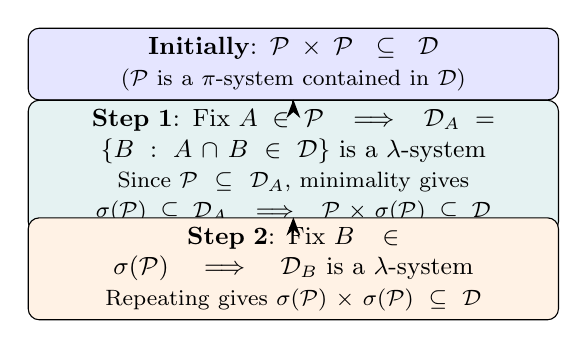
\begin{tikzpicture}[font=\small, >=Stealth]
  \node[draw, rounded corners, fill=blue!10, text width=6.5cm, align=center] (B0) at (0, 2.6)
    {\textbf{Initially}: $\mathcal{P} \times \mathcal{P} \subseteq \mathcal{D}$ \\ \footnotesize ($\mathcal{P}$ is a $\pi$-system contained in $\mathcal{D}$)};
  \node[draw, rounded corners, fill=teal!10, text width=6.5cm, align=center] (B1) at (0, 1.3)
    {\textbf{Step 1}: Fix $A \in \mathcal{P} \implies \mathcal{D}_A = \{B: A \cap B \in \mathcal{D}\}$ is a $\lambda$-system \\ \footnotesize Since $\mathcal{P} \subseteq \mathcal{D}_A$, minimality gives $\sigma(\mathcal{P}) \subseteq \mathcal{D}_A \implies \mathcal{P} \times \sigma(\mathcal{P}) \subseteq \mathcal{D}$};
  \node[draw, rounded corners, fill=orange!10, text width=6.5cm, align=center] (B2) at (0, 0.0)
    {\textbf{Step 2}: Fix $B \in \sigma(\mathcal{P}) \implies \mathcal{D}_B$ is a $\lambda$-system \\ \footnotesize Repeating gives $\sigma(\mathcal{P}) \times \sigma(\mathcal{P}) \subseteq \mathcal{D}$};

  \draw[->, thick] (B0) -- (B1);
  \draw[->, thick] (B1) -- (B2);
\end{tikzpicture}
\end{document}